\chapter{Implementierung}
\label{ch:implementation}

In diesem Kapitel wird die Implementierung der Anwendung beschrieben.
% Hierbei wird exemplarisch auf zwei wichtige Funktionen der Anwendung eingegangen.
% Diese sind die Verwaltung des Benutzerprofils und die Erstellung und Anzeige von Beiträgen.

Da der komplette Code und viele Screenshots den Rahmen dieses Kapitels sprengen würden, wird in den einzelnen Kapiteln nur ein Auszug gezeigt.
Den kompletten Code findet man direkt im Github Repository unter \url{https://github.com/Jonasdero/digital-hometown-frontend}.


\section{Landing-Page}
\label{sec:landing_page}

Bei dem Aufruf der Plattform \glqq Digital Dahoam\grqq \ wird der Nutzer auf die Landing-Page (s. \autoref{fig:landing_page}) weitergeleitet. Diese ist abhängig davon, ob der Nutzer eingeloggt ist oder nicht.

Auf der Landing-Page wird die Vision der Plattform vorgestellt. Bei dem Projekt \glqq Digital Dahoam\grqq \ geht es darum, dass sich Menschen in der Nachbarschaft vernetzen können. Die Plattform soll zudem die Menschen dazu motivieren, anderen zu helfen, bzw. selbst um Hilfe zu bitten. Insbesondere für neu zugezogene Menschen soll die Plattform eine Möglichkeit sein, die Umgebung zu entdecken und interessante Vereine kennenzulernen.

\begin{figure}[!htb]
  \centering
  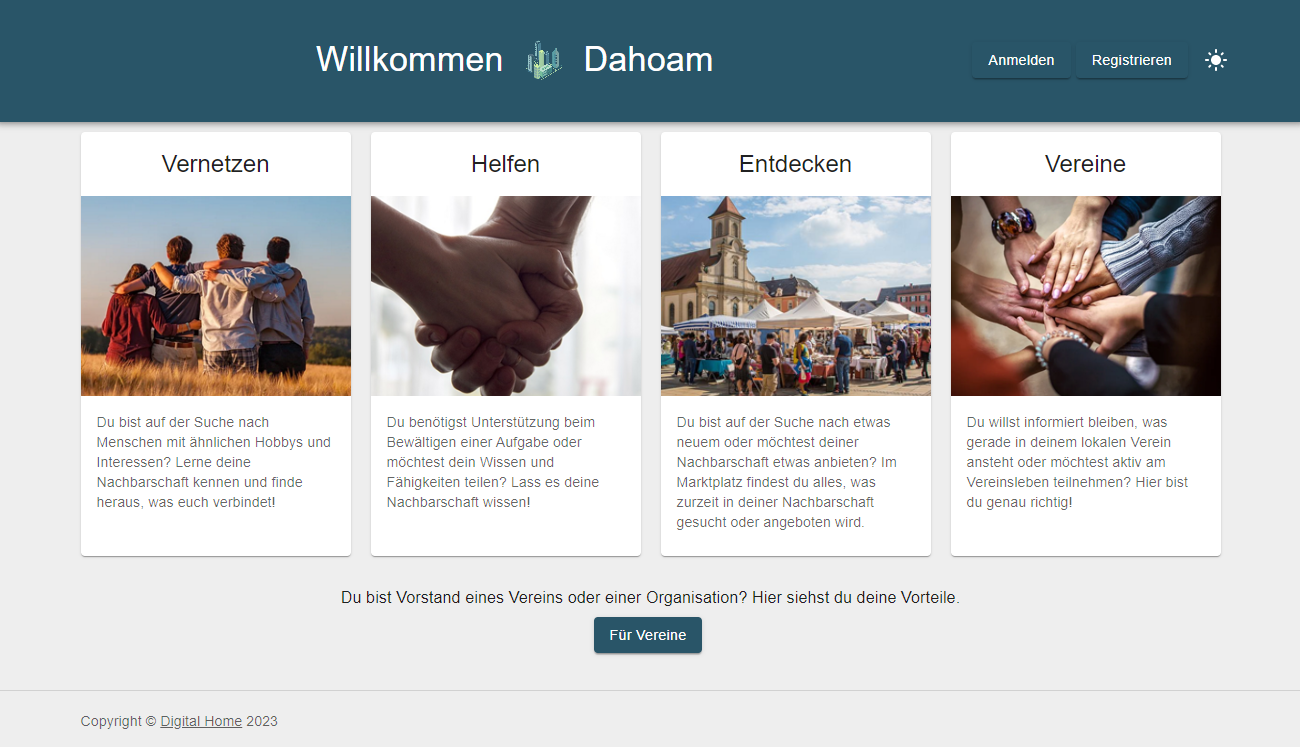
\includegraphics[width=.9\textwidth]{figures/boas/21_landing_page.png}
  \caption[]{Bildschirmaufnahme der Startseite für nicht eingeloggte Nutzer}
  \label{fig:landing_page}
\end{figure}

Will sich ein Benutzer bspw. ein Vereinsvorstand mit seinem Verein registrieren, kann er über den Button \glqq Für Vereine\grqq \ zur Landing Page für Vereine navigieren. Über die Landing Page für Vereine kann der Vorstand seinen Verein bei der Plattform registrieren oder sich einloggen (s. \autoref{fig:landing_page_verein}). Der Inhalt der Landing Page beschreibt, welche Vorteile die Plattform für Vereine bietet.


\begin{figure}[!htb]
  \centering
  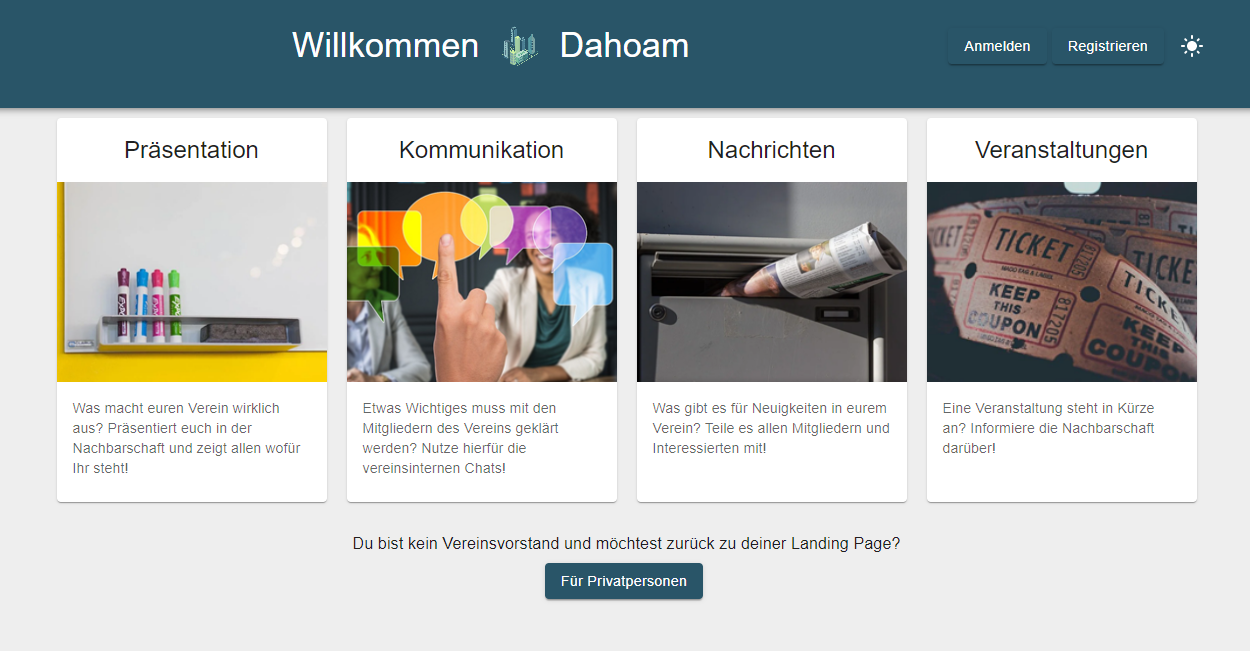
\includegraphics[width=.9\textwidth]{figures/boas/21_landing_page_verein.png}
  \caption[]{Bildschirmaufnahme der Startseite für nicht eingeloggte Vereine}
  \label{fig:landing_page_verein}
\end{figure}

Wenn der Benutzer eingeloggt ist, wird er auf das Dashboard weitergeleitet, das aktuelle Beiträge und Veranstaltungen anzeigt.

Da die Landing-Page eine statische Seite darstellt, wird hier nicht weitere auf die Implementierung eingegangen.


\section{Profil}
\label{sec:profile}

Die Profile eines Nutzers sind in der Anwendung sehr wichtig.
Jeder Nutzer verwaltet sein eigenes Profil, welches er mit anderen Nutzern teilt.
Dazu gehören Informationen wie Name, E-Mail-Adresse, Geburtsdatum, Geschlecht und ein Profilbild.
Damit andere Nutzer die Informationen des Profils sehen können, muss das Profil öffentlich sein.
Zudem sollen Benutzer der Anwendung durch Interessen, Profilbilder und persönliche Beschreibungen voneinander unterscheidbar sein und sich so besser vernetzen können.
Um sich mit anderen Nutzern zu verbinden, ist es wichtig, dass diese Informationen in der Anwendung gespeichert werden.

Außerdem soll die soziale Interaktion zwischen Nutzer ermöglicht werden.
Dazu gehören Funktionen wie das Folgen von anderen Nutzern oder auch das Schreiben von Nachrichten zwischen zwei Nutzern oder in Gruppen.
Dies soll direkt vom Profil eines Nutzers aus möglich sein.

\begin{figure}[ht!]
  \begin{centering}
    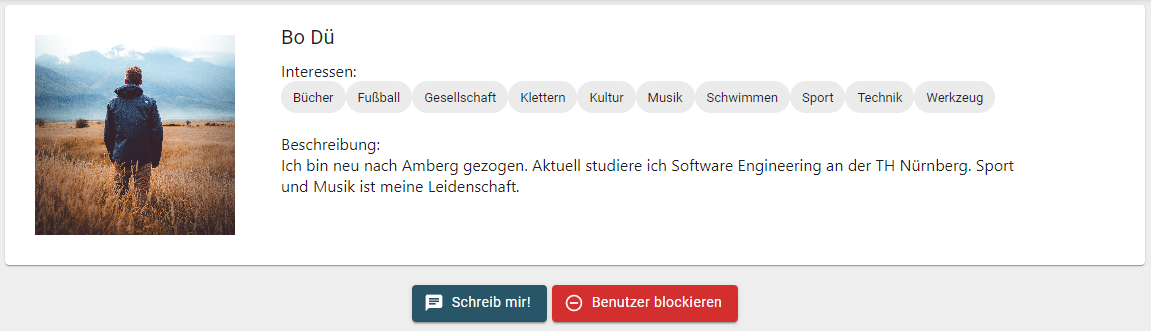
\includegraphics[width=1\textwidth]{figures/implementation/profile-header.png}
    \caption{Übersicht eines Benutzerprofils}
    \label{fig:userProfileHeader}
  \end{centering}
\end{figure}

Hier sieht man die verschiedenen Informationen, die ein Nutzer in seinem Profil angeben kann.
In den nächsten Seiten wird die Implementierung dieser Funktionen beschrieben.
Diese wird aufgeteilt in die verschiedenen Bereiche: \textit{Anmeldung \& Registrierung}, \textit{persönliches Accountmanagement}, \textit{Profilseite \& Profilbilder} und \textit{blockierte Nutzer}.

\subsection{Anmeldung \& Registrierung}
\label{sec:login}

Den Nutzern wird die Möglichkeit gegeben, sich mit einer E-Mail-Adresse und einem Passwort anzumelden oder eine direkte Anmeldung über OAuth mit Google zu nutzen.
Dies wird beides durch die Firebase Authentication API ermöglicht.

Sobald ein Nutzer sich registriert hat, wird von Firebase intern ein Benutzerprofil erstellt, welches wichtige Nutzermetadaten und Authentifizierungsinformationen enthält.
Außerdem wird bei der Anmeldung über Google das Profilbild mit in Firebase gespeichert.
Die Anmeldemaske sieht wie folgt aus:

\begin{figure}[ht!]
  \begin{centering}
    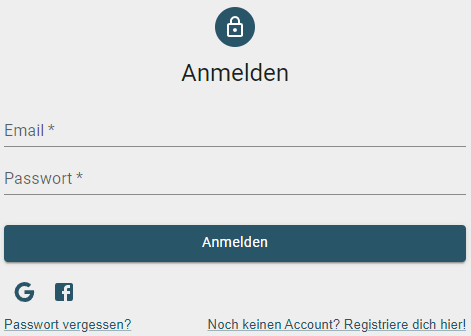
\includegraphics[width=.75\textwidth]{figures/implementation/anmeldemaske.png}
    \caption{Anmeldemaske}
    \label{fig:login}
  \end{centering}
\end{figure}

Um diese Daten in der Anwendung zu speichern, wird ein eigener Benutzerdatensatz angelegt, sobald ein Nutzer registriert wurde und Daten aus dem internen Benutzerprofil von Firebase mit übertragen.
Hierbei wird unterschieden, ob der aktuelle Benutzer ein normaler Nutzer oder ein Verein ist.
Diese werden in unterschiedlichen „Collections“ gespeichert.
Bei der Anmeldung wird dann geprüft, welchen Typ der Benutzer hat und die Daten entsprechend geladen.
Dadurch kann mit einer Datenstruktur gearbeitet werden, die für beide Typen geeignet ist.
Andere Ansichten basieren dann häufig auf der Unterscheidung zwischen Nutzern und Vereinen.
Die Struktur des Datensatzes kann man in Abbildung \ref{fig:firestoreUser} sehen.

\section{Authentifizierung}
\label{sec:authentifizierung}

Essentiell für ein soziales Netzwerk ist es, dass die Benutzer sich mit einem Profil registrieren können. Wie das im Detail funktioniert und wie die Authentifizierung implementiert wurde, wird in diesem Kapitel beschrieben.

\subsection{Verwendung des \glqq Firebase-Authentication\grqq-Services}
\label{sec:firebase_authentifizierung}
Die Implementierung der Authentifizierung wird mit dem Backend-as-a-Service-Anbieter Firebase durchgeführt. Firebase bietet eine Schnittstelle, die es ermöglicht, Profile anzulegen sowie den Anmelde- und Registrierungsprozess mit wenigen Zeilen Code zu implementieren.

Durch die verschiedenen Authentifizierungsmethoden, die Firebase anbietet, kann der Nutzer sich mit E-Mail und Passwort, Google oder Facebook anmelden. Die Authentifizierungsmethoden können einfach in der Firebase-Konsole aktiviert werden.

Es wird zu dem die Möglichkeit geboten, dass Nutzer, die ihre Zugangsdaten vergessen haben, eine E-Mail mit einem Link zum Zurücksetzen des Passworts erhalten.

Die Beschriebenen Funktionen decken also einen standardmäßigen Anmelde- und Registrierungsprozess ab.

\subsection{Zugriff auf die Profilinformationen}
\label{sec:zugriff_profilinformationen}
Wie bei der React-Einführung beschrieben, ist es aufwendig, Informationen wie die des Profils über die gesamte Anwendung hinweg durchzureichen. Dafür wurde auch bereits die Möglichkeit des React Contexts vorgestellt. Da dieses Konzept auch für die Profilinformationen eingesetzt wird hier nochmal ein Beispiel der Implementierung gezeigt.

Das in \autoref{lst:authcontext} stellt das Interface des Contexts dar, das für alle Components befüllt wird. Die Profilinformationen sind im Attribute \texttt{currentUser} gespeichert.

\begin{lstlisting}[language=JavaScript, caption=Auszug aus dem Interface des Authentifizierungscontexts, label={lst:authcontext}]
interface AuthContextI {
  currentUser: User | Club | undefined | null
  setCurrentUser: React.Dispatch<React.SetStateAction<User | Club | undefined | null>>
  logOut: () => void
  logIn: (email: string, password: string) => void
  signUpWithEmail: (email: string, password: string, displayName: string, isOrg: boolean) => Promise<void>
  signUpOAuth: (providerName: "google" | "facebook", isOrg: boolean) => void
  // usw.
}
\end{lstlisting}

% \autocite{attlassian2023}
Um den Vorteil des Contexts für die Codequalität hervorzuheben wird in \autoref{lst:authcontext_impl} dargestellt, wie einfach es möglich ist, die zentral befüllten Attribute in einer beliebigen React-Komponente zu verwenden.
Hierbei wird das Prinzip der Higher-Order-Components (HOC) genutzt, das zuvor implementiert wurde. Es ist lediglich notwendig, die implementierte Komponente mit dem HOC \texttt{withAuth} zu umschließen. Dieses HOC stellt der jeweiligen Komponente die Attribute des Contexts als Props zur Verfügung.

\begin{lstlisting}[language=JavaScript, caption=Verwendung des Authentifizierungscontext-HOCs, label={lst:authcontext_impl}]
function SignOut({ logOut }: AuthContextI) {
  useEffect(() => logOut(), [logOut])
  return <Navigate to="/" />
}

export default withAuth(SignOut)  
\end{lstlisting}

Das Component \texttt{SignOut} bekommt hier beispielsweise durch das HOC automatisch die Funktion \texttt{logOut} als Prop übergeben, die dann zum Ausloggen des Benutzers verwendet wird.

\subsection{Authentifizierungsprozess}
\label{sec:authentifizierungsprozess}

Im folgenden wird nun anhand von Bildschirmaufnahmen gezeigt, wie der Authentifizierungsprozess abläuft.

Beim Klick auf den Registrieren-Button der Landing-Page wird man auf eine Seite weitergeleitet, über die Benutzername, Email und Passwort eingegeben werden können (s. \autoref{fig:registrierung}). Fehlerhafte Eingaben der E-Mail-Adresse, sowie die redundante Eingabe des Passworts werden hierbei validiert.

\begin{figure}[!htb]
  \centering
  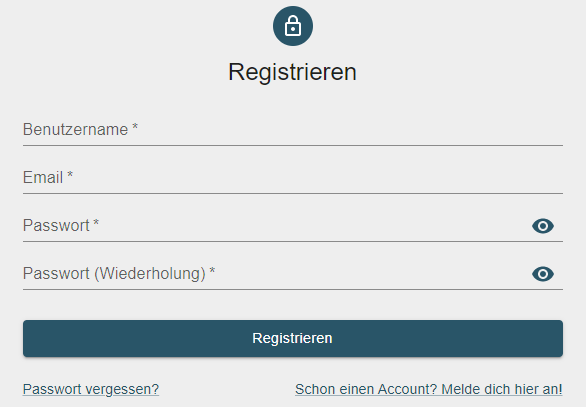
\includegraphics[width=0.5\textwidth]{figures/boas/21_registrieren.png}
  \caption[]{Registrierungsseite}
  \label{fig:registrierung}
\end{figure}

Nach der erfolgreichen Registrierung des Nutzers, wird er zunächst auf eine Seite geführt, auf der er seine Profilinformationen um das Geburtsdatum und die Postleitzahl ergänzen kann (s. \autoref{fig:registrieren_profilinfo}).

\begin{figure}[htb]
  \centering
  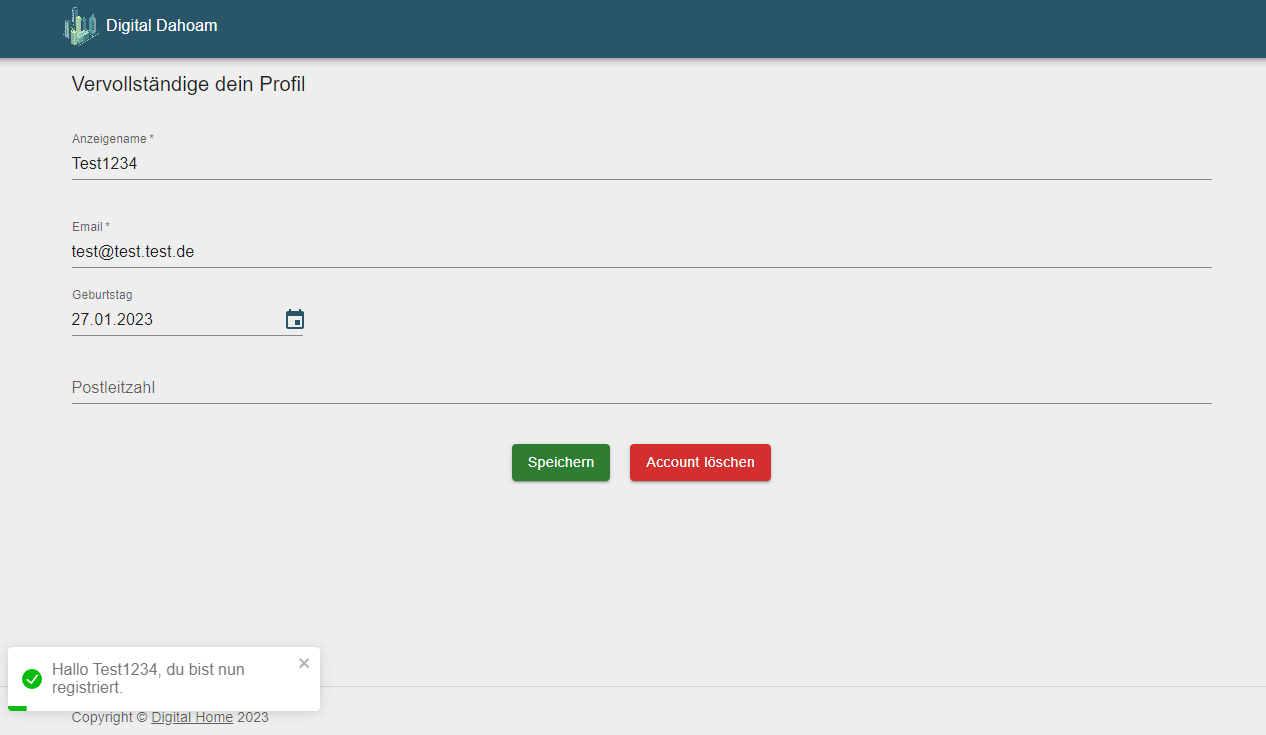
\includegraphics[width=0.9\textwidth]{figures/boas/21_registrieren_profilinfo.png}
  \caption[]{Ergänzen der Profilinformationen beim ersten Anmelden}
  \label{fig:registrieren_profilinfo}
\end{figure}

Nach der erfolgreichen Registrierung wird der Nutzer auf sein Profil weitergeleitet, wo er u. a. Interessen hinterlegen kann, um von Nutzern gefunden zu werden, welche die gleichen Interessen haben. Details hierzu sind in \autoref{sec:profilepictures} beschrieben.

Eine besonders einfache Möglichkeit, sich bei der Plattform zu registrieren, bzw. anzumelden ist die Authentifizierung über Google. Beim Klick auf das Google-Icon öffnet sich direkt der Google-OAuth-Dialog (s. \autoref{fig:anmelden_google}). Dies steigert die Usability der Plattform, da der Nutzer nicht mehr die E-Mail-Adresse und das Passwort eingeben muss.

\begin{figure}[htb]
  \centering
  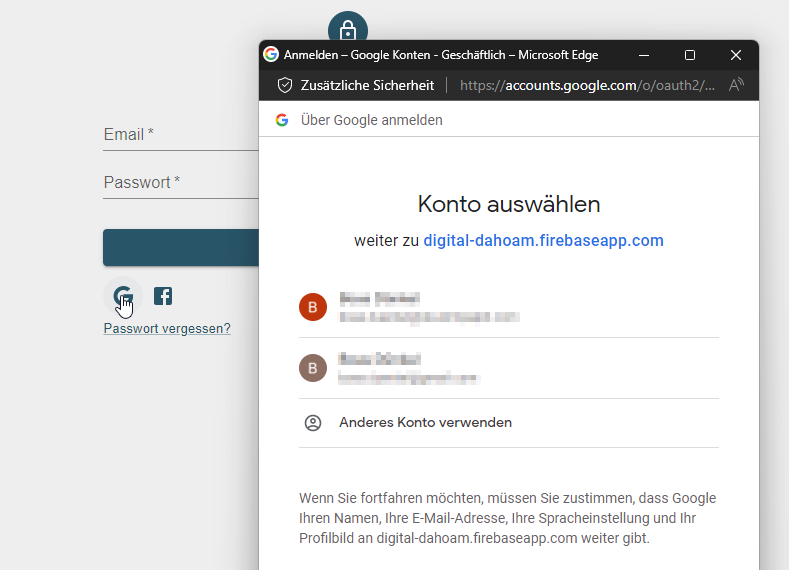
\includegraphics[width=0.6\textwidth]{figures/boas/21_anmelden_google.png}
  \caption[]{Authentifizierungs-Dialog beim Anmelden mit Google}
  \label{fig:anmelden_google}
\end{figure}

Wenn der Nutzer sich mit einer E-Mail-Adresse registriert hat, kann er sich auf folgender Seite anmelden (s. \autoref{fig:anmeldung}).

\begin{figure}[htb]
  \centering
  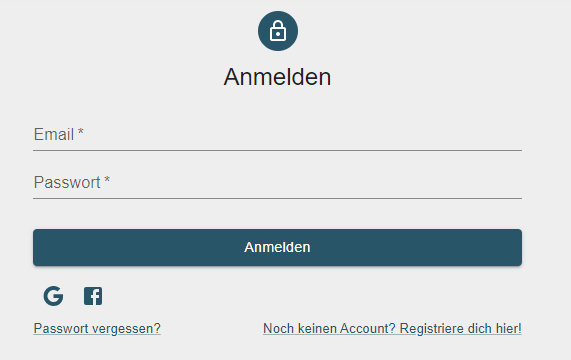
\includegraphics[width=0.5\textwidth]{figures/boas/21_anmelden.png}
  \caption[]{Anmeldeseite}
  \label{fig:anmeldung}
\end{figure}

\clearpage

\subsection{Persönliches Accountmanagement}
\label{sec:accountmanagement}

Um die Daten des Benutzerprofils zu verwalten, gibt es eine Seite, auf der der Nutzer seine persönlichen Daten ändern kann.
Diese werden dann in der Anwendung aktualisiert und in der Datenbank gespeichert. Er hat hier die Möglichkeit seinen Namen, seine E-Mail, sein Geburtsdatum und seine Postleitzahl zu ändern.
Hier kann außerdem der komplette Account gelöscht werden, um die Daten des Nutzers zu löschen.

\begin{figure}[ht!]
  \begin{centering}
    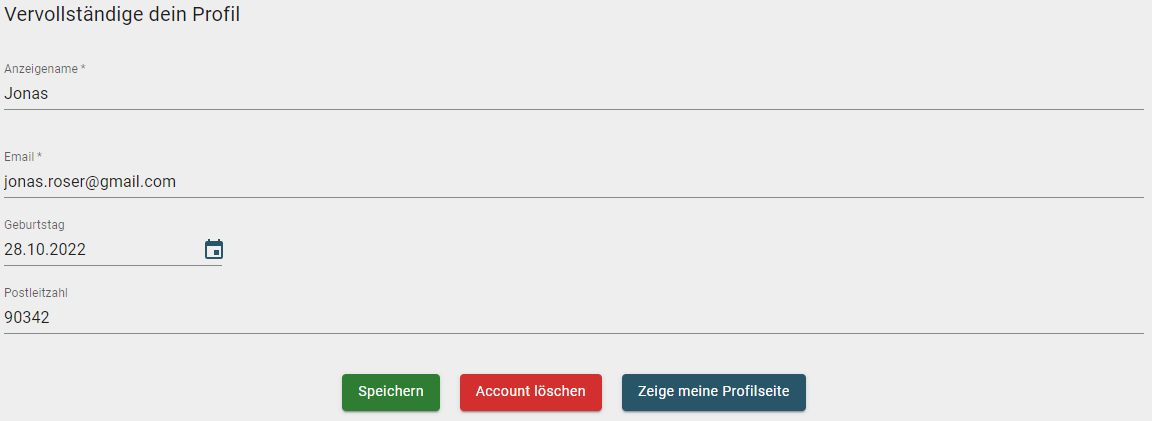
\includegraphics[width=1\textwidth]{figures/implementation/userSettings.png}
    \caption{Benutzereinstellungen}
    \label{fig:userSettings}
  \end{centering}
\end{figure}

\subsection{Profilseite \& Profilbilder}
\label{sec:profilepictures}

Auf der Profilseite des Nutzers kann er seine persönlichen Daten einsehen und bearbeiten. Hier können Interessen und eine Beschreibung hinzugefügt werden.
Außerdem kann er sein Profilbild ändern, indem er auf das Profilbild oder auf den Knopf mit der Kamera klickt.
Dies wird dann im Firebase Storage gespeichert und in der Datenbank verlinkt.

Das Ganze ist so aufgebaut, dass Nutzer zwischen einer Vorschau, also der Sicht, die auch andere Nutzer von seinem Profil sehen und der Bearbeitungssicht unterscheiden können.

\begin{figure}[ht!]
  \begin{centering}
    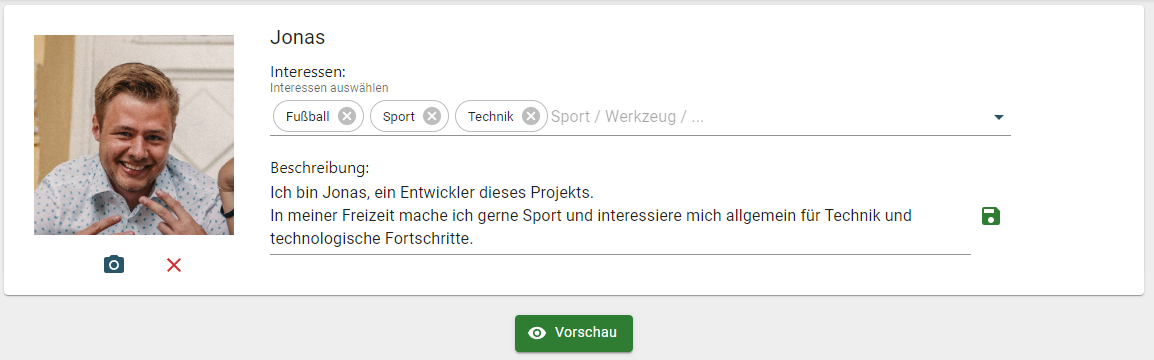
\includegraphics[width=1\textwidth]{figures/implementation/my-profile-header.png}
    \caption{Persönliches Profil}
    \label{fig:myProfileHeader}
  \end{centering}
\end{figure}

\subsection{Blockierte Nutzer}
\label{sec:blockedusers}

Um die Privatsphäre der Nutzer zu schützen, können diese andere Nutzer blockieren.
Blockierte Nutzer können dann nicht mehr auf das Profil des Blockierenden zugreifen und auch keine Nachrichten mehr schreiben.

Über die Profilseite kann ein Nutzer einen anderen Nutzer blockieren.

\begin{figure}[ht!]
  \begin{centering}
    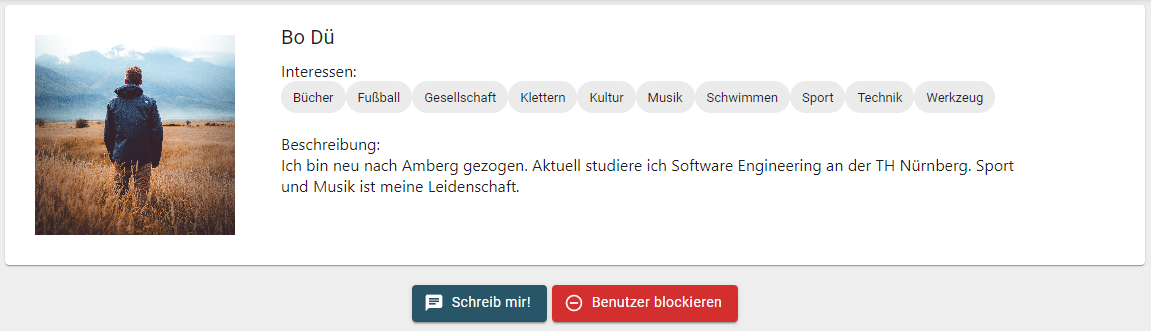
\includegraphics[width=1\textwidth]{figures/implementation/profile-header.png}
    \caption{Blockieren eines Nutzers}
    \label{fig:blockUser}
  \end{centering}
\end{figure}

Blockierte Nutzer kann man dann in der Anwendung unter dem Menüpunkt \textit{Blockiert} einsehen.
Dort wird jeder Nutzer oder Verein aufgeführt, welcher blockiert ist.
Mit einem Klick auf das „X“ wird der Block aufgehoben.

\begin{figure}[ht!]
  \begin{centering}
    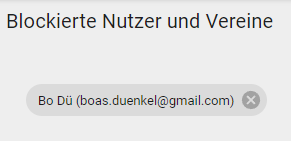
\includegraphics[width=.5\textwidth]{figures/implementation/blocked.png}
    \caption{Blockierte Nutzer}
    \label{fig:blocked}
  \end{centering}
\end{figure}

\section{Beiträge}
\label{sec:contributions}

Beiträge sind ein anderes wichtiges Feature von „Digital Dahoam“.
Hiermit können Nutzer Informationen austauschen, die für andere Nutzer interessant sein könnten.
Beiträge können von allen Nutzern erstellt werden, die sich registriert haben.
Es gibt folgende Typen von Beiträgen:

\begin{itemize}
  \item \textbf{Anfrage}: Hier können Nutzer eine Anfrage stellen, die dann von anderen Nutzern beantwortet werden kann. Anfragen können auch benutzt werden, wenn bestimmte Gegenstände im Haushalt fehlen, z. B. ein bestimmtes Werkzeug oder ein bestimmtes Lebensmittel.
  \item \textbf{Angebot}: Hier können Nutzer ein Angebot erstellen, das dann von anderen Nutzern angenommen werden kann. Dies kann wie Ebay-Kleinanzeigen benutzt werden, um überflüssige Gegenstände zu verkaufen.
  \item \textbf{Information}: Hier können Nutzer Informationen teilen, die für andere Nutzer interessant sein könnten.
  \item \textbf{Veranstaltung}: Hier können Nutzer Veranstaltungen erstellen, die dann von anderen Nutzern besucht werden können.
\end{itemize}

\subsection{Beiträge erstellen}
\label{sec:createpost}

Beiträge können mit einem Klick auf den Button \textit{Beiträge erstellen} erstellt werden.
Hier öffnet sich ein Pop-up, welchem der Nutzer den Titel, die Beschreibung, den Beitragstyp und die Kategorie des Beitrags eingeben kann.
Außerdem werden für jeden Beitrag das Startdatum, also ab wann der Beitrag gültig ist und angezeigt wird, und das Enddatum, also bis wann der Beitrag gültig ist und angezeigt wird, festgelegt.
Für Veranstaltungen gibt es zusätzlich noch den Ort und das Datum.
Sobald auf \textit{absenden} geklickt wird, wird der Beitrag in der Datenbank gespeichert und auf der Startseite angezeigt.

\begin{figure}[ht!]
  \begin{centering}
    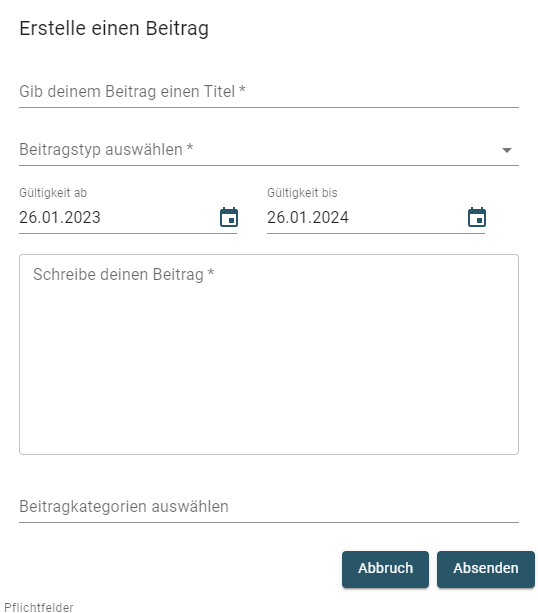
\includegraphics[width=.65\textwidth]{figures/implementation/createpost.png}
    \caption{Beiträge erstellen}
    \label{fig:createpost}
  \end{centering}
\end{figure}


\subsection{Alle Beiträge}
\label{sec:allposts}

Unter \textit{Alle Beiträge} findet man alle Beiträge, die ein valides Gültigkeitsdatum haben. Diese werden mit Titel, Beschreibung, Kategorie und Beitragstyp angezeigt.
Für Veranstaltungen gibt es zusätzlich noch den Ort und das Datum.

\begin{figure}[ht!]
  \begin{centering}
    
\includegraphics[width=.8\textwidth]{figures/implementation/beitrag.png}
    \caption{Beitrag}
    \label{fig:beitrag}
  \end{centering}
\end{figure}

Ein Problem, was es während der Implementierung zu lösen galt, war die richtige Filterung der Beiträge. Die hier verwendete Sortierfunktion (siehe \ref{code:filterPosts}) wurde dann für die restlichen Listen verwendet und die gefilterten Beiträge dort nur noch verfeinert.
Diese musste folgendes erfüllen:

\begin{itemize}
  \item Eigene Beiträge werden immer angezeigt.
  \item Beiträge, die nicht mehr gültig sind, werden nicht angezeigt.
  \item Beiträge von blockierten Nutzern werden nicht angezeigt.
  \item Beiträge müssen nach Datum sortiert werden.
\end{itemize}

Mit dem Klick auf die 3 kleinen Punkte in der rechten oberen Ecke öffnet man das Beitragsmenü. Hier gibt es folgende Punkte:

\begin{itemize}
  \item \textbf{Beitrag zum Merkzettel}: Hinzufügen eines Inhalts zum Merkzettel.
  \item \textbf{Details}: Anzeigen der Details des Beitrags. (siehe \ref{fig:details})
  \item \textbf{Zum Autor}: Direkter Link zum Profil des Autors.
  \item \textbf{Nachricht an Autor}: Direkter Link zur Nachrichtenfunktion, um dem Autor eine Nachricht zu schicken.
\end{itemize}

\begin{figure}[ht!]
  \begin{centering}
    \includegraphics[width=.25\textwidth]{figures/implementation/beitragsmenü.png}
    \caption{Beitragsmenü}
    \label{fig:beitragsmenü}
  \end{centering}
\end{figure}

\clearpage
\subsection{Profilseite}
\label{sec:profilepage}

Auf der Profilseite kann der Nutzer werden seine Beiträge angezeigt.
Hier werden auch abgelaufene Beiträge angezeigt und grau hinterlegt.

\begin{figure}[ht!]
  \begin{centering}
    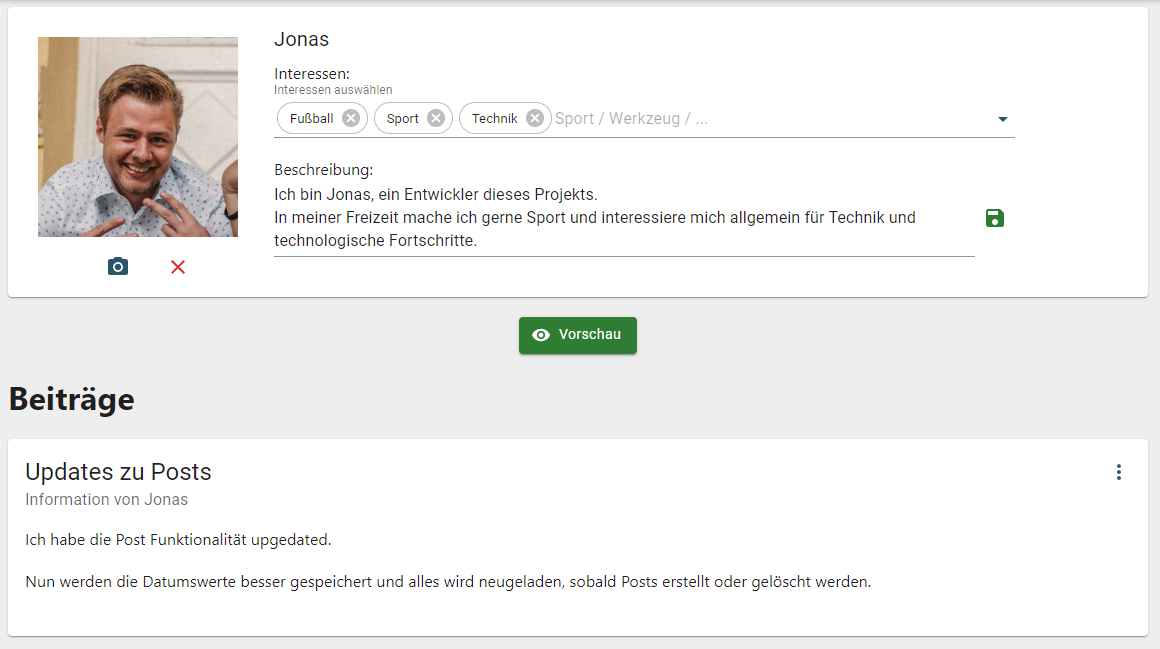
\includegraphics[width=1\textwidth]{figures/implementation/userposts.png}
    \caption{Beiträge des Nutzers}
    \label{fig:userposts}
  \end{centering}
\end{figure}

\subsection{Merkzettel}
\label{sec:bookmark}

Beiträge, die für den Merkzettel markiert sind erscheinen dort, und können dort auch wieder entfernt werden.
Außerdem werden sie nach Beitragstyp gruppiert.

\begin{figure}[ht!]
  \begin{centering}
    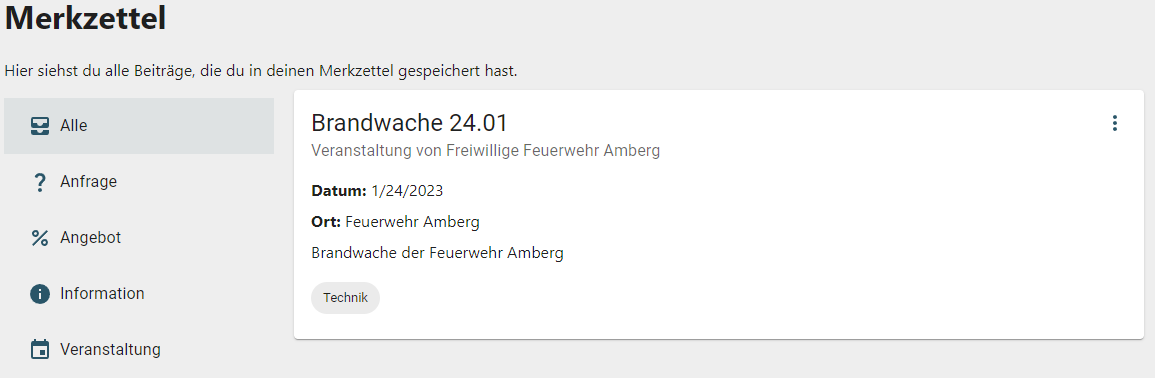
\includegraphics[width=1\textwidth]{figures/implementation/merkzettel.png}
    \caption{Merkzettel}
    \label{fig:merkzettel}
  \end{centering}
\end{figure}

\clearpage
\subsection{Marktplatz}
\label{sec:marketplace}

Auf dem Marktplatz können Personen und Beiträge durchsucht werden.
Durch den Filter auf Kategorien, Informationen oder Veranstaltungen findet man schnell den richtigen Beitrag.

\begin{figure}[ht!]
  \begin{centering}
    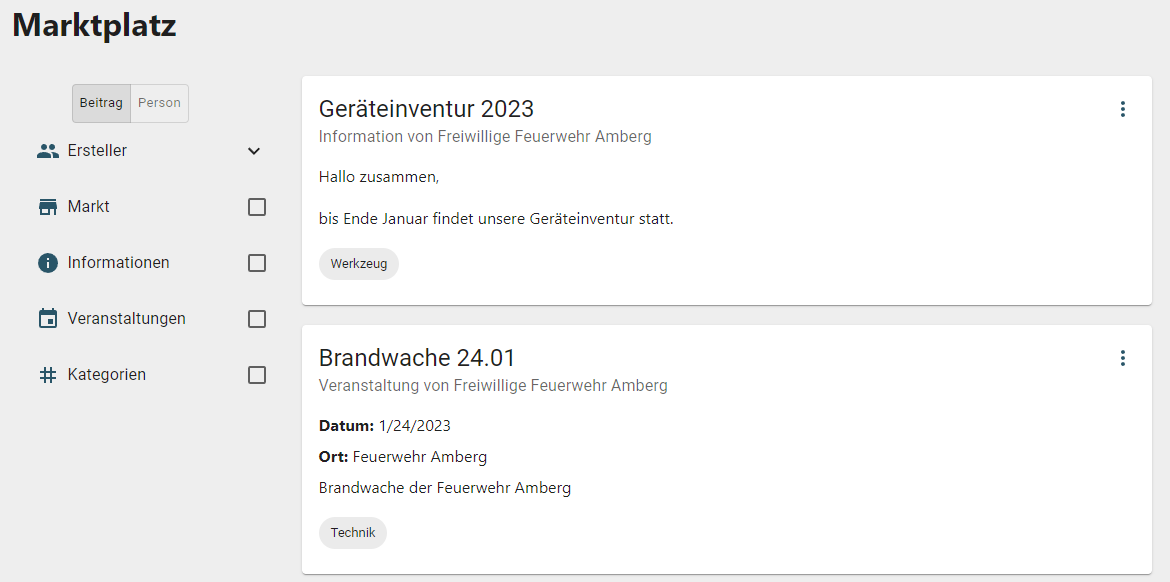
\includegraphics[width=1\textwidth]{figures/implementation/marktplatz.png}
    \caption{Marktplatz}
    \label{fig:marktplatz}
  \end{centering}
\end{figure}


\subsection{Dashboard}
\label{sec:dashboard}

Auf der Startseite werden aktuelle Beiträge aus der Nähe angezeigt, sowie die Veranstaltungen, die der Nutzer auf dem Merkzettel hat.

\begin{figure}[ht!]
  \begin{centering}
    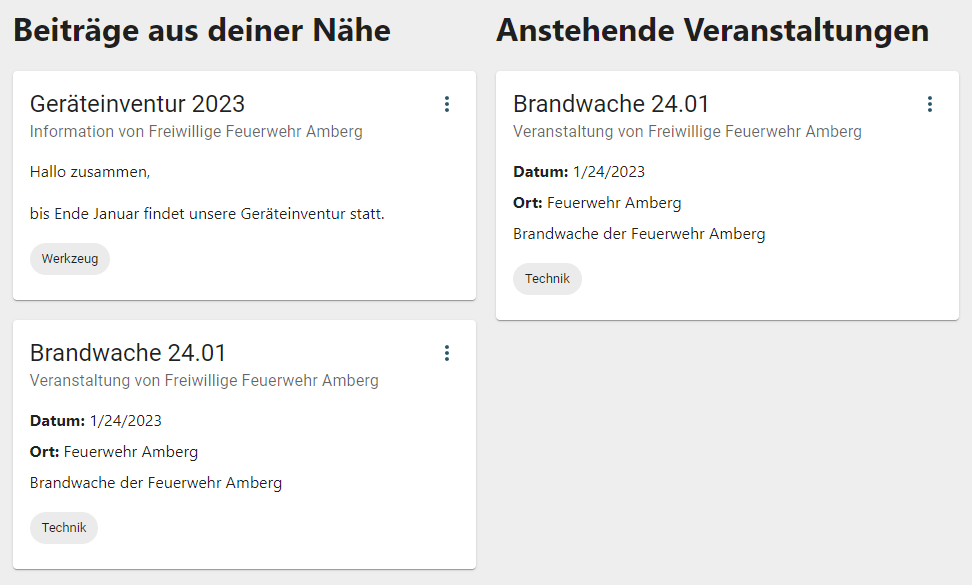
\includegraphics[width=.8\textwidth]{figures/implementation/dashboard.png}
    \caption{Dashboard}
    \label{fig:dashboard}
  \end{centering}
\end{figure}

\section{Chat}
\label{sec:chat}

Ein wichtiges Tool für das soziale Netzwerk \glqq Digital Hometown\grqq \ ist der Chat, da hier die Personen in Kontakt treten und sich austauschen können.

Auf technischer Ebene sind für einen Chat mehrere Technologien erforderlich, wodurch die Umsetzung nicht trivial ist. Neben den Laden der Bereits gesendeten Nachrichten und dem Absenden von Nachrichten, ist es für eine gute Usability notwendig, dass neue Nachrichten sofort bei allen Chatteilnehmern sichtbar sind. Diese Anforderung kann in effizienter Weise durch die Verwendung von bidirektionalen WebSocket-Verbindungen ermöglicht werden.

\subsection{Firebase Realtime Database für den Chat}
\label{sec:firebase_realtime_db_chat}

Für den Chat wird die Firebase Realtime Database (Realtime DB) verwendet. Dadurch wird die Implementierung deutlich vereinfacht, da die entsprechende JavaScript Bibliothek einfach in die React Anwendung integriert werden kann. Eine Echtzeitsynchronisation zwischen den Clients (Browseranwendungen der User) und der Datenbank kann mit geringem Aufwand umgesetzt werden. Die Realtime DB ist eine NoSQL Datenbank.
Die Firebase DB wird in diesem Projekt ausschließlich für den Chat verwendet und hat dabei zwei Hauptwurzelelemente (s. \autoref{fig:hauptwurzel_realtime_db}) verwendet werden. Bei dem Design wurde darauf geachtet, dass die einzelnen Hauptwurzelelemente keine zu große Verschachtelung aufweisen, um eine gute Performanz zu gewährleisten.

\begin{figure}[!htb]
  \centering
  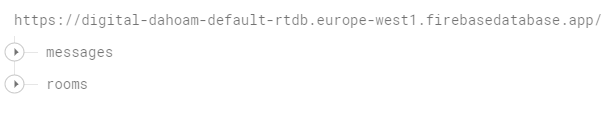
\includegraphics[width=0.8\textwidth]{figures/boas/21_hauptwurzel_realtime_db.png}
  \caption[]{Hauptwurzelelemente der Realtime DB}
  \label{fig:hauptwurzel_realtime_db}
\end{figure}


\subsection{Autorisierung der Nachrichten und Chaträume}
\label{sec:autorisierung_chat}
Eine wichtige Anforderung für die Implementierung einer Chatfunktionalität ist es, dass Nachrichten nur von Mitgliedern des jeweiligen Chatraums gelesen werden können. Dies wird mit den Realtime DB Regeln umgesetzt. Ein Auszug hiervon ist in \autoref{lst:rules_realtime_db} dargestellt. Kurz zusammengefasst ermöglicht diese Konfiguration, dass nur Nachrichten von Benutzern gelesen und geschrieben werden können, die ein Mitglied des Chatraumes sind.

\begin{lstlisting}[language=JavaScript, caption=Realtime DB Regeln für Chatnachrichten, label={lst:rules_realtime_db}]
{
  "rules": {
    "messages": {
      "$roomUid": {
        ".read": "root.child('rooms/' + $roomUid + '/members').hasChild(auth.uid)",
        ".write": "root.child('rooms/' + $roomUid + '/members').hasChild(auth.uid)"
      },
      "messages": {
        ".indexOn": "sendAt"
      }
    },
    ...
  }
}
\end{lstlisting}

\subsection{Benutzung des Chats}
\label{sec:benutzung_chat}

Im folgenden wird anhand von Screenshots die Benutzung des Chats beschrieben. \autoref{fig:chat_screenshot} zeigt die Standardansicht des Chats. Auf der linken Seite sind die Chaträume aufgelistet. Die Chaträume sind in zwei Kategorien unterteilt. Zum einen gibt es die Chaträume, die mit Einzelpersonen erstellt wurden und zum anderen die Chaträume mit mehreren Personen (Gruppenchats). In der Liste der Chaträume werden Gruppenchats mit einem Gruppenicon hervorgehoben.

\begin{figure}[!htb]
  \centering
  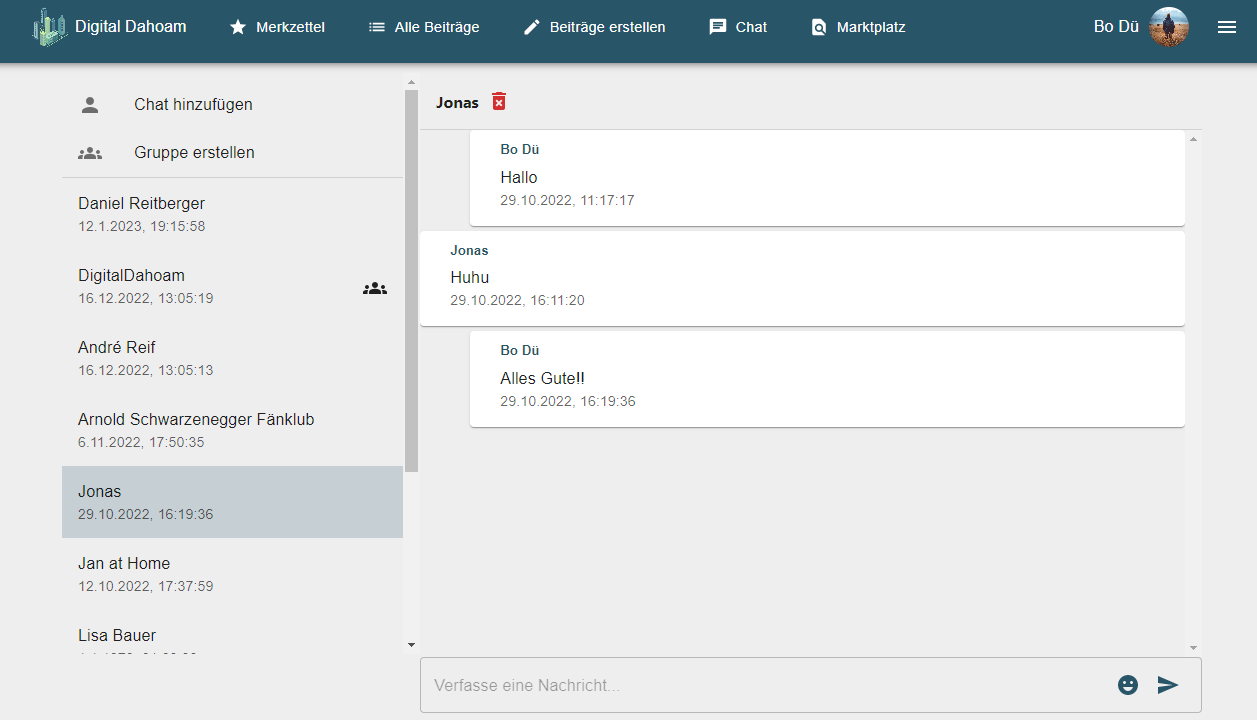
\includegraphics[width=1\textwidth]{figures/boas/21_chat.png}
  \caption[]{Ansicht des Chats in der Anwendung}
  \label{fig:chat_screenshot}
\end{figure}

Über den Button \glqq Chat hinzufügen\grqq \ wir die in \autoref{fig:new_personal_chat} dargestellte Ansicht geöffnet, wo alle Personen der Plattform angezeigt werden. Hier kann ein neuer Chat mit einer Einzelperson erstellt werden.

\begin{figure}[!htb]
  \centering
  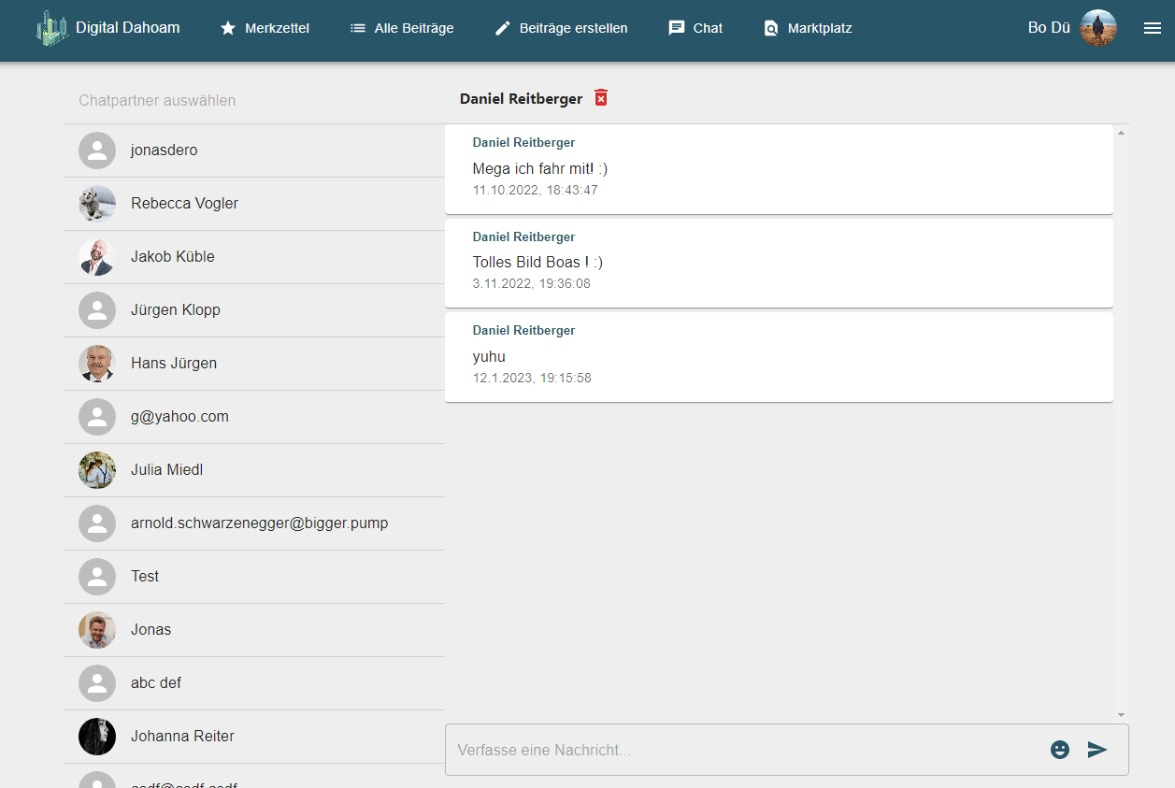
\includegraphics[width=.9\textwidth]{figures/boas/21_new_chat.jpeg}
  \caption[]{Hinzufügen von Chats mit Einzelpersonen}
  \label{fig:new_personal_chat}
\end{figure}

Das Hinzufügen von Gruppenchats erfolgt über den Button \glqq Gruppe hinzufügen\grqq. Der Ablauf sieht hier wie folgt aus. Zuerst wird automatisch ein neuer Chatraum erstellt. Wird dieser ausgewählt, lässt sich über einen Button die in \autoref{fig:edit_chat_group} dargestellte Ansicht öffnen. Hier können die Mitglieder des Chatraumes hinzugefügt werden, indem die entsprechenden Personen aus der Liste ausgewählt werden. Es besteht zudem die Möglichkeit, der Chatgruppe einen anderen Namen zu geben.

\begin{figure}[!htb]
  \centering
  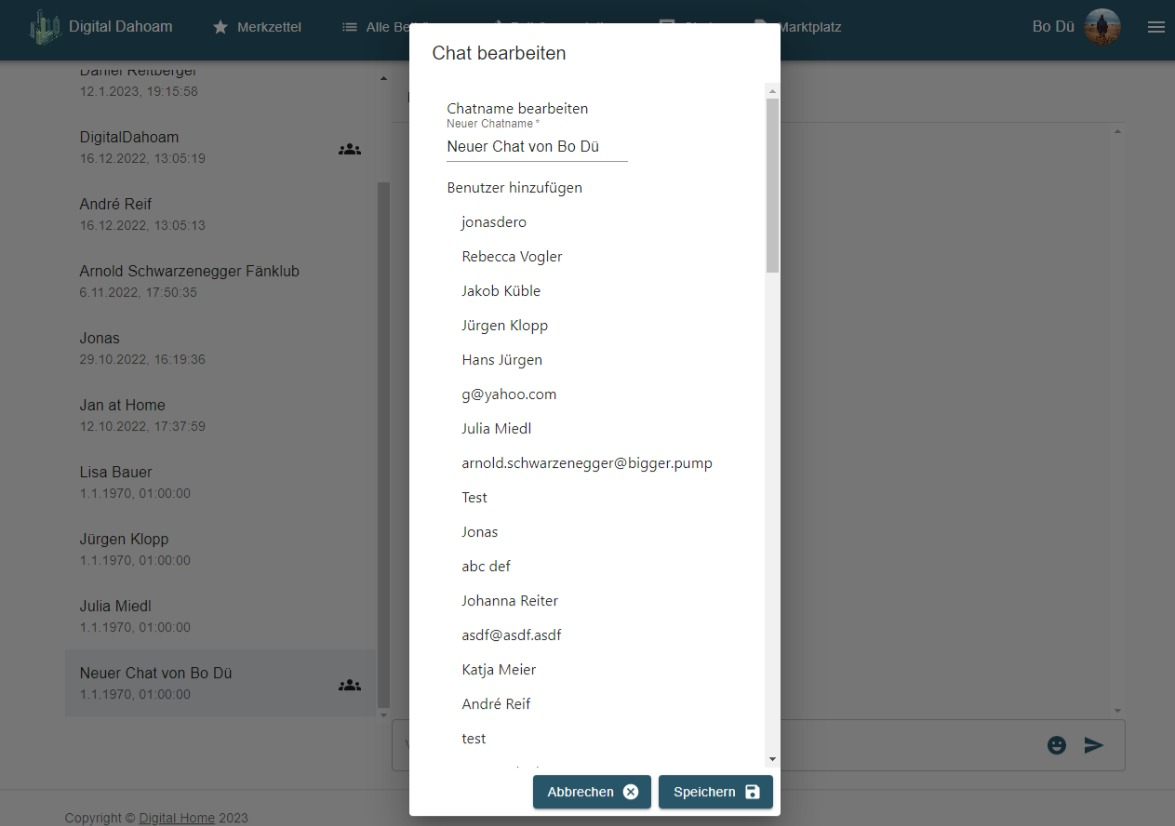
\includegraphics[width=.9\textwidth]{figures/boas/21_edit_chat_group.jpeg}
  \caption[]{Chatgruppe umbenennen und Mitglieder hinzufügen}
  \label{fig:edit_chat_group}
\end{figure}

\subsection{Verknüpfung von Beitragen mit dem Chatraum des Beitragautors}
\label{sec:beitrag_chat_verknüpfung}

Die Motivation des in diesem Absatz beschriebenen Features wird mit folgendem Fallbeispiel erläutert.

Angenommen, ein Benutzer meldet sich an, da er an Fußball interessiert ist und gerne mit Menschen aus seiner Nachbarschaft gerne zum Fußball spielen treffen möchte. Er sieht nun einen Beitrag, der genau diesem Bedürfnis entspricht. Wie in \autoref{fig:beitrag_nachricht} dargestellt, kann er nun über den Button \glqq Nachricht an Autor\grqq direkt zum Chatraum des Beitragautors gelangen. Dort kann er den Beitragautor anschreiben und sich mit ihm zum Fußball spielen treffen.

\begin{figure}[!htb]
  \centering
  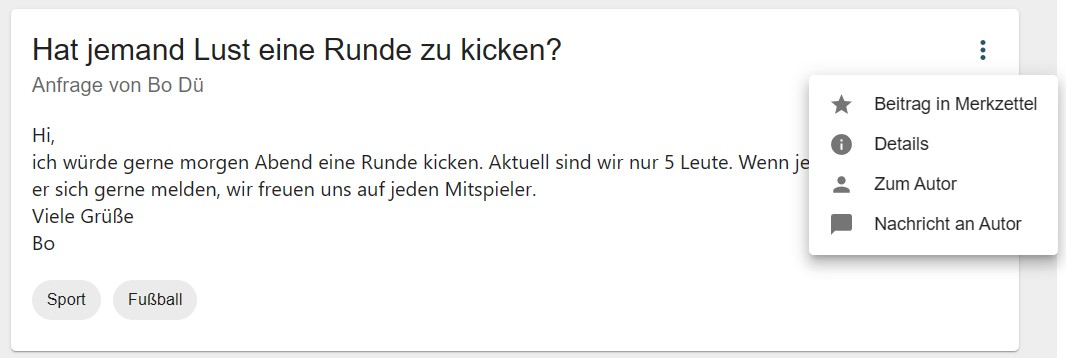
\includegraphics[width=.7\textwidth]{figures/boas/21_beitrag_nachricht.jpg}
  \caption[]{Möglichkeit von einem Beitrag direkt zum Chatraum des Beitragautors zu gelangen}
  \label{fig:beitrag_nachricht}
\end{figure}

Im Hintergrund muss dafür der gemeinsame Chatraum ermittelt werden. Falls dieser noch nicht existiert, muss er erstellt werden. Wird dann der Nutzer auf die Chatseite weitergeleitet, öffnet sich automatisch der entsprechende Chatraum.
